\documentclass[11pt]{article}
\usepackage[top=2cm,bottom=2cm,left=2cm,right= 2cm]{geometry}
%\geometry{landscape}                % Activate for for rotated page geometry
\usepackage[parfill]{parskip}    % Activate to begin paragraphs with an empty line rather than an indent
\usepackage{graphicx}
\usepackage{amssymb}
\usepackage{epstopdf}
\usepackage{amsmath}            
\usepackage{multirow}    
\usepackage{changepage}
\usepackage{lscape}
\usepackage{ulem}
\usepackage{multicol}
\usepackage{dashrule}
\usepackage[usenames,dvipsnames]{color}       
\usepackage{enumerate}
\newcommand{\urlwofont}[1]{\urlstyle{same}\url{#1}}
\newcommand{\degree}{\ensuremath{^\circ}}

\DeclareGraphicsRule{.tif}{png}{.png}{`convert #1 `dirname #1`/`basename #1 .tif`.png}

\newenvironment{choices}{
\begin{enumerate}[(a)]
}{\end{enumerate}}

%\newcommand{\soln}[1]{\textcolor{MidnightBlue}{\textit{#1}}}	% delete #1 to get rid of solutions for handouts
\newcommand{\soln}[1]{ \vspace{2.7cm} }

\newcommand{\solnMult}[1]{\textbf{\textcolor{MidnightBlue}{\textit{#1}}}}	% uncomment for solutions
%\newcommand{\solnMult}[1]{ #1 }	% uncomment for handouts

%\newcommand{\pts}[1]{ \textbf{{\footnotesize \textcolor{black}{(#1)}}} }	% uncomment for handouts
\newcommand{\pts}[1]{ \textbf{{\footnotesize \textcolor{red}{(#1)}}} }	% uncomment for handouts

\newcommand{\note}[1]{ \textbf{\textcolor{red}{[#1]}} }	% uncomment for handouts

\definecolor{oiG}{rgb}{.298,.447,.114}
\definecolor{oiB}{rgb}{.337,.608,.741}

\usepackage[colorlinks=false,pdfborder={0 0 0},urlcolor= oiG,colorlinks=true,linkcolor= oiG, citecolor= oiG,backref=true]{hyperref}

%\usepackage{draftwatermark}
%\SetWatermarkScale{4}

\usepackage{titlesec}
\titleformat{\section}
{\color{oiB}\normalfont\Large\bfseries}
{\color{oiB}\thesection}{1em}{}
\titleformat{\subsection}
{\color{oiB}\normalfont}
{\color{oiB}\thesubsection}{1em}{}

\newcommand{\ttl}[1]{ \textsc{{\LARGE \textbf{{\color{oiB} #1} } }}}

\newcommand{\tl}[1]{ \textsc{{\large \textbf{{\color{oiB} #1} } }}}

\begin{document}

Dr. \c{C}etinkaya-Rundel \hfill Data Analysis and Statistical Inference \\

\ttl{Application exercise: \\
1.3 Distributions of numerical variables} 

\section{Shapes of distributions}

\begin{enumerate}

\item Below are two histograms. One corresponds to the age at which a sample of people applied for marriage licenses; the other corresponds to the last digit of a sample of social security numbers. Which graph is which, and why?

\begin{multicols}{2}

\begin{enumerate}

\item $\:$ \\
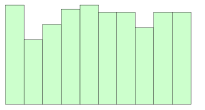
\includegraphics[height=1.2in]{last_digit_SSN}

\item $\:$ \\
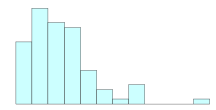
\includegraphics[height=1.2in]{age_mar_lic}

\end{enumerate}

\end{multicols}

%

\item Match the following variables with the histograms and bar graphs given below. These data represent Sta 101 students at Duke. [\textit{Hint: Think about how each variable should behave.}]

\begin{multicols}{2}
\begin{enumerate}
\item the height of students
\item gender breakdown of students
\item the time it took students to get to their first class of the day
\item the number of hours of sleep students received last night
\item whether or not students live off campus
\item the number of piercings students have
\end{enumerate}
\end{multicols}


\begin{multicols}{3}

\begin{enumerate}[(1)]

\item $\:$ \\
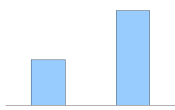
\includegraphics[height=1.2in]{gender}

\item $\:$ \\
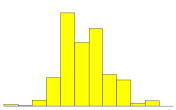
\includegraphics[height=1.2in]{height}

\item $\:$ \\
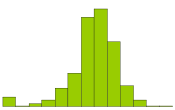
\includegraphics[height=1.2in]{sleep}

\item $\:$ \\
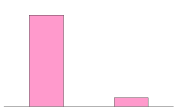
\includegraphics[height=1.2in]{off_campus}

\item $\:$ \\
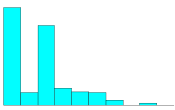
\includegraphics[height=1.2in]{piercings}

\item $\:$ \\
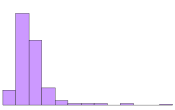
\includegraphics[height=1.4in]{time_to_class}

\end{enumerate}

%

\end{multicols}

\item Come up with a concise way (1-2 sentences) to teach someone how to determine the expected distribution of any variable.

\end{enumerate}

%

\section{Variability}

\begin{enumerate}

\item Order histograms A, B, and C from least to most variable. Explain your reasoning.

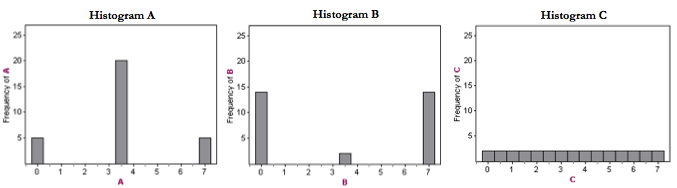
\includegraphics[width=\textwidth]{histogramsVarOrderABC}

$\:$ \\
$\:$ \\
$\:$ \\

\item Between histograms D and E, which exhibits more variability? Explain your reasoning.

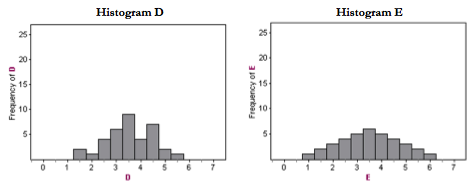
\includegraphics[width=\textwidth]{histogramsVarOrderDE}

\end{enumerate}

%

\end{document}